\chapter{Spectroscopy}
In this chapter we present results of searches of binding energies and wave functions in the way proposed by Deng et al.~\cite{deng-bot,deng-charm}. For testing purposes we use bottomonium along with charmonium. Bottomonium consists of heavier quarks so non-relativistic quark model applies better to it (compare to charmonium~\cref{fig:charm-states}). We use the following values of model parameters provided by Deng et al.~\cite{deng-bot,deng-charm}:

\begin{table} \begin{floatrow}
\ttabbox
    {\caption{Parameters used for charmonium}}
    {\begin{tabular}{l|c|c}
        {} & Linear & Screened \\ \hline
        Parameter & {} & {} \\ \cline{1-1}
        $\alpha_S$ & 0.5461 & 0.5070 \\
        $b$ [$GeV^2$] & 0.1425 & 0.2100 \\
        $m_c$ [$GeV$] & 1.4830 & 1.4110 \\
        $\sigma$ [$GeV$] & 1.1384 & 1.1600 \\
        $r_C$ [$fm$] & 0.202 & 0.180 \\
        $\mu$ [$GeV$] & \ldots & 0.0979 \\ \hline
    \end{tabular}}
\hspace{2cm}
\ttabbox
    {\caption{Parameters used for bottomonium}}
    {\begin{tabular}{l|c}
        {} & Screened \\ \hline
        Parameter & {} \\ \cline{1-1}
        $\alpha_S$ & 0.368 \\
        $b$ [$GeV^2$] & 0.206 \\
        $m_b$ [$GeV$] & 4.757 \\
        $\sigma$ [$GeV$] & 3.10 \\
        $r_C$ [$fm$] & 0.060 \\
        $\mu$ [$GeV$] & 0.056 \\ \hline
    \end{tabular}}
\end{floatrow}
\end{table}

\begin{figure}[H]
    \centering
    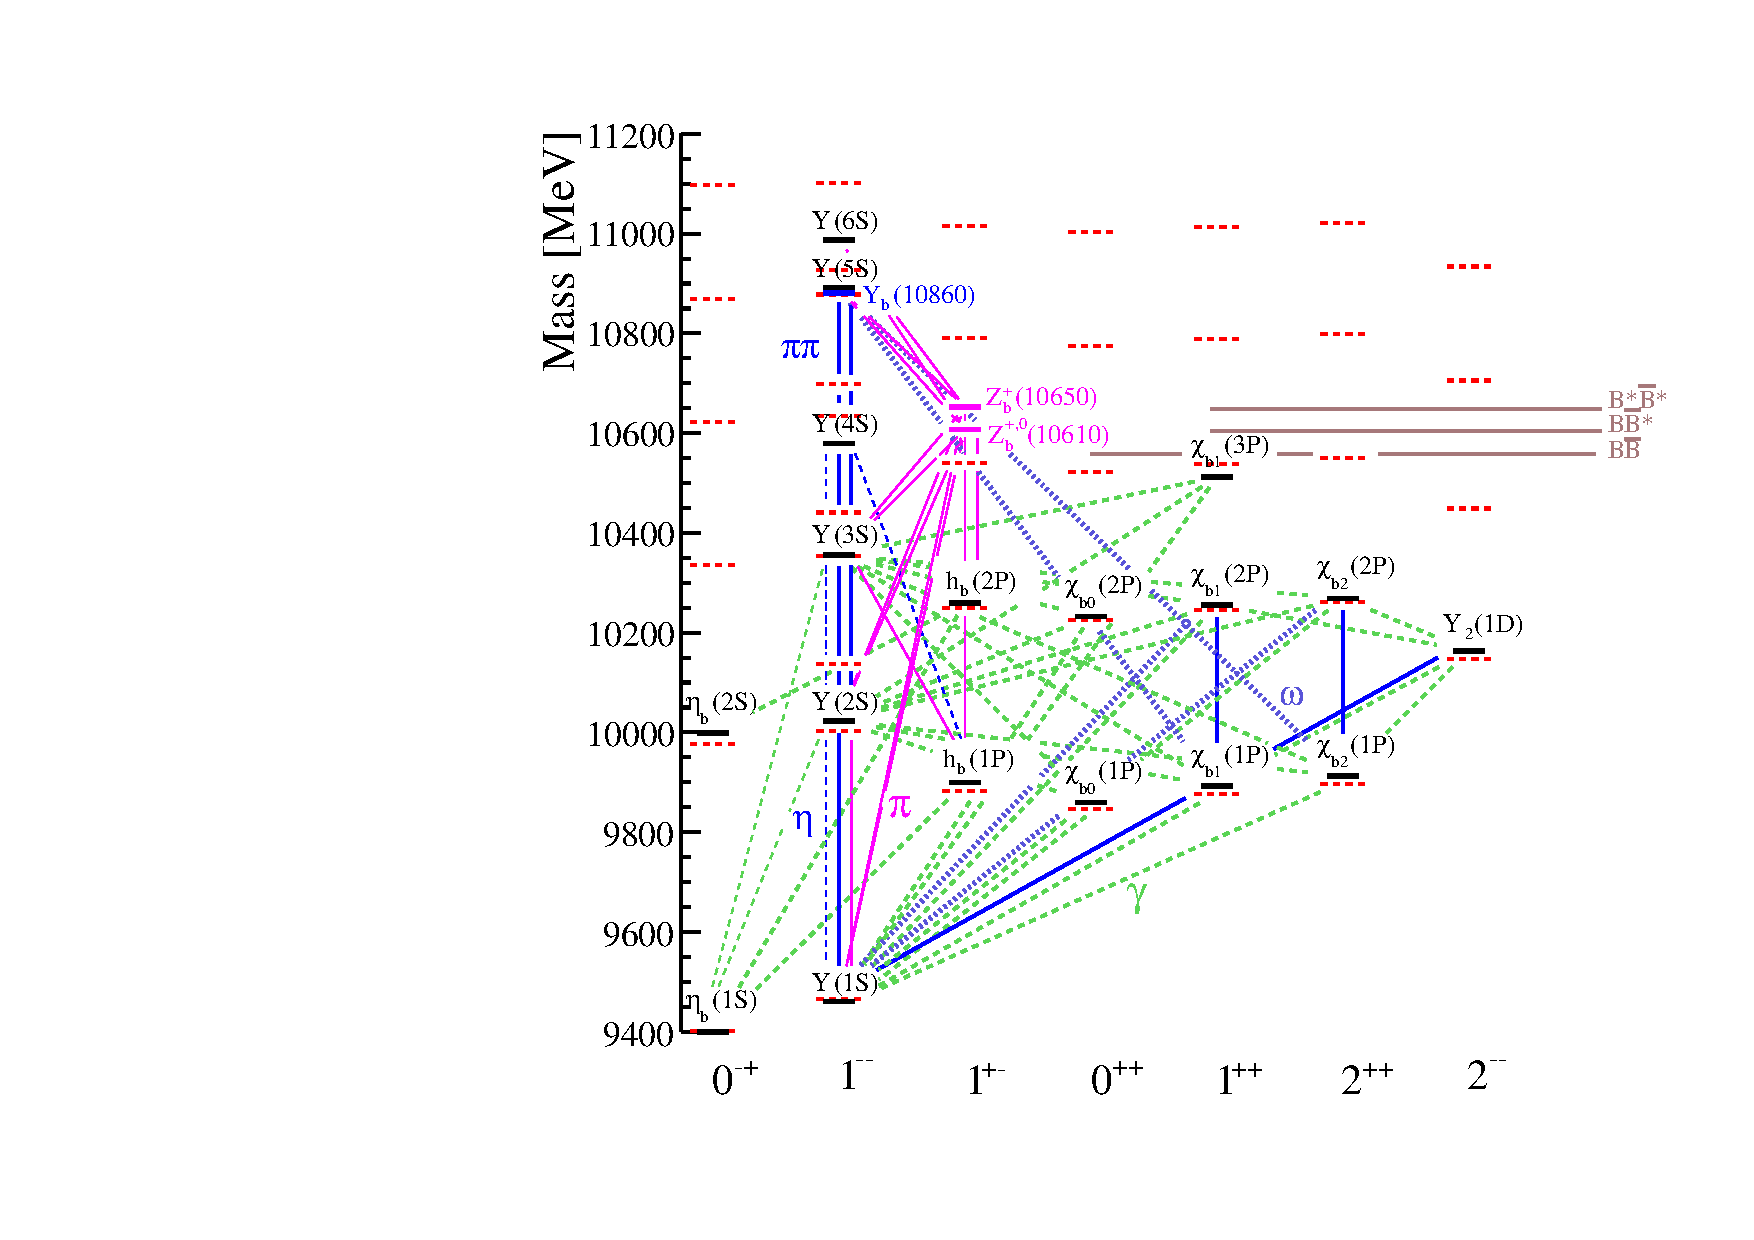
\includegraphics[width=15cm]{bottomoniumExotic.pdf}
    \caption{The status of bottomonium spectrum in August 2017. Red dashed lines represent theoretical predictions based on Godfrey-Isgur model with relativistic corrections to higher-excited states~\cite{gbs-model}. Black solid lines are experimentally measured energy levels. Here are also shown measured transitions. We are interested in radiative transitions which are represented by green dashed lines: thick for E1 and thin for M1. Source: Olsen, Skwarnicki, Zieminska~\cite{heavy-quark_pics}} \label{fig:bot-states}
\end{figure}

The method of searching for binding energies is based on the fact that eigenfunctions of Shrodinger equation should be localized, i.e. swiftly go to zero when far from origin. Especially for screened potential one can express asymptotic solution of  the radial equation(\cref{eq:nrqm-radialeq}) as a linear combination of exponents.

\begin{align}
    &\dv[2]{u(r)}{r} + 2 \mu_R \left[ E_{bound} - V(r) - \frac{L(L+1)}{2 \mu_R r^2} \right] u(r) = 0 \\
    &u(r) \approx C_+ \ee^{k r} + C_- \ee^{-k r},\qquad k = \sqrt{2 \mu_R E}
\end{align}

Exponent with negative sign will vanish at infinity, but positive exponent will grow enormously. The only way how to suppres the growth --- put $C_+ = 0$. Both $C_+$ and $C_-$ are functions of binding energy, so equality of $C_+(E) = 0$ is a direct criterion for $E$ being an eigenvalue.

The method uses information about wave function magnitude at infinity, so we have to be able to solve Shrodinger equation for any value of $E$ as a parameter. The equation is of the second order without first derivatiive. Gowell quadrature~\cite{deng-bot} comes in handy here, because to conduct the next step it doesn't need first derivative (which we don't know, but can only approximate with a first difference). Methods making use of the ``first difference'' usually worked well initially but failed at distant points, supposingly due to an error growth implied by inaccurate first derivative approximation. 

To show the idea of how the process looks like on practice we provide a plot of $C_+$ as a function of mass of the state. Notice the sharp dip near the $M$ corresponding to the eigestate. Numerically it is hard to find exact zero of $C_+$, for that one needs am infinite precision. What we really look for --- damping of the value of $C_+$ by some factor. This factor is related to precision with which we know the eigenvalue. For example, in case of $\chi_{b0}(1P)$ we apply damping by factor $10^{10}$, and from width of dips one can estimate precision by order of magnitude. Roughly, each factor $10^{2}$ for $C_+$ corresponds to fixation of a digit in the value of the eigenvalue, after $10^{10}$ we expect precision to $100~KeV$:

\begin{figure}[H]
    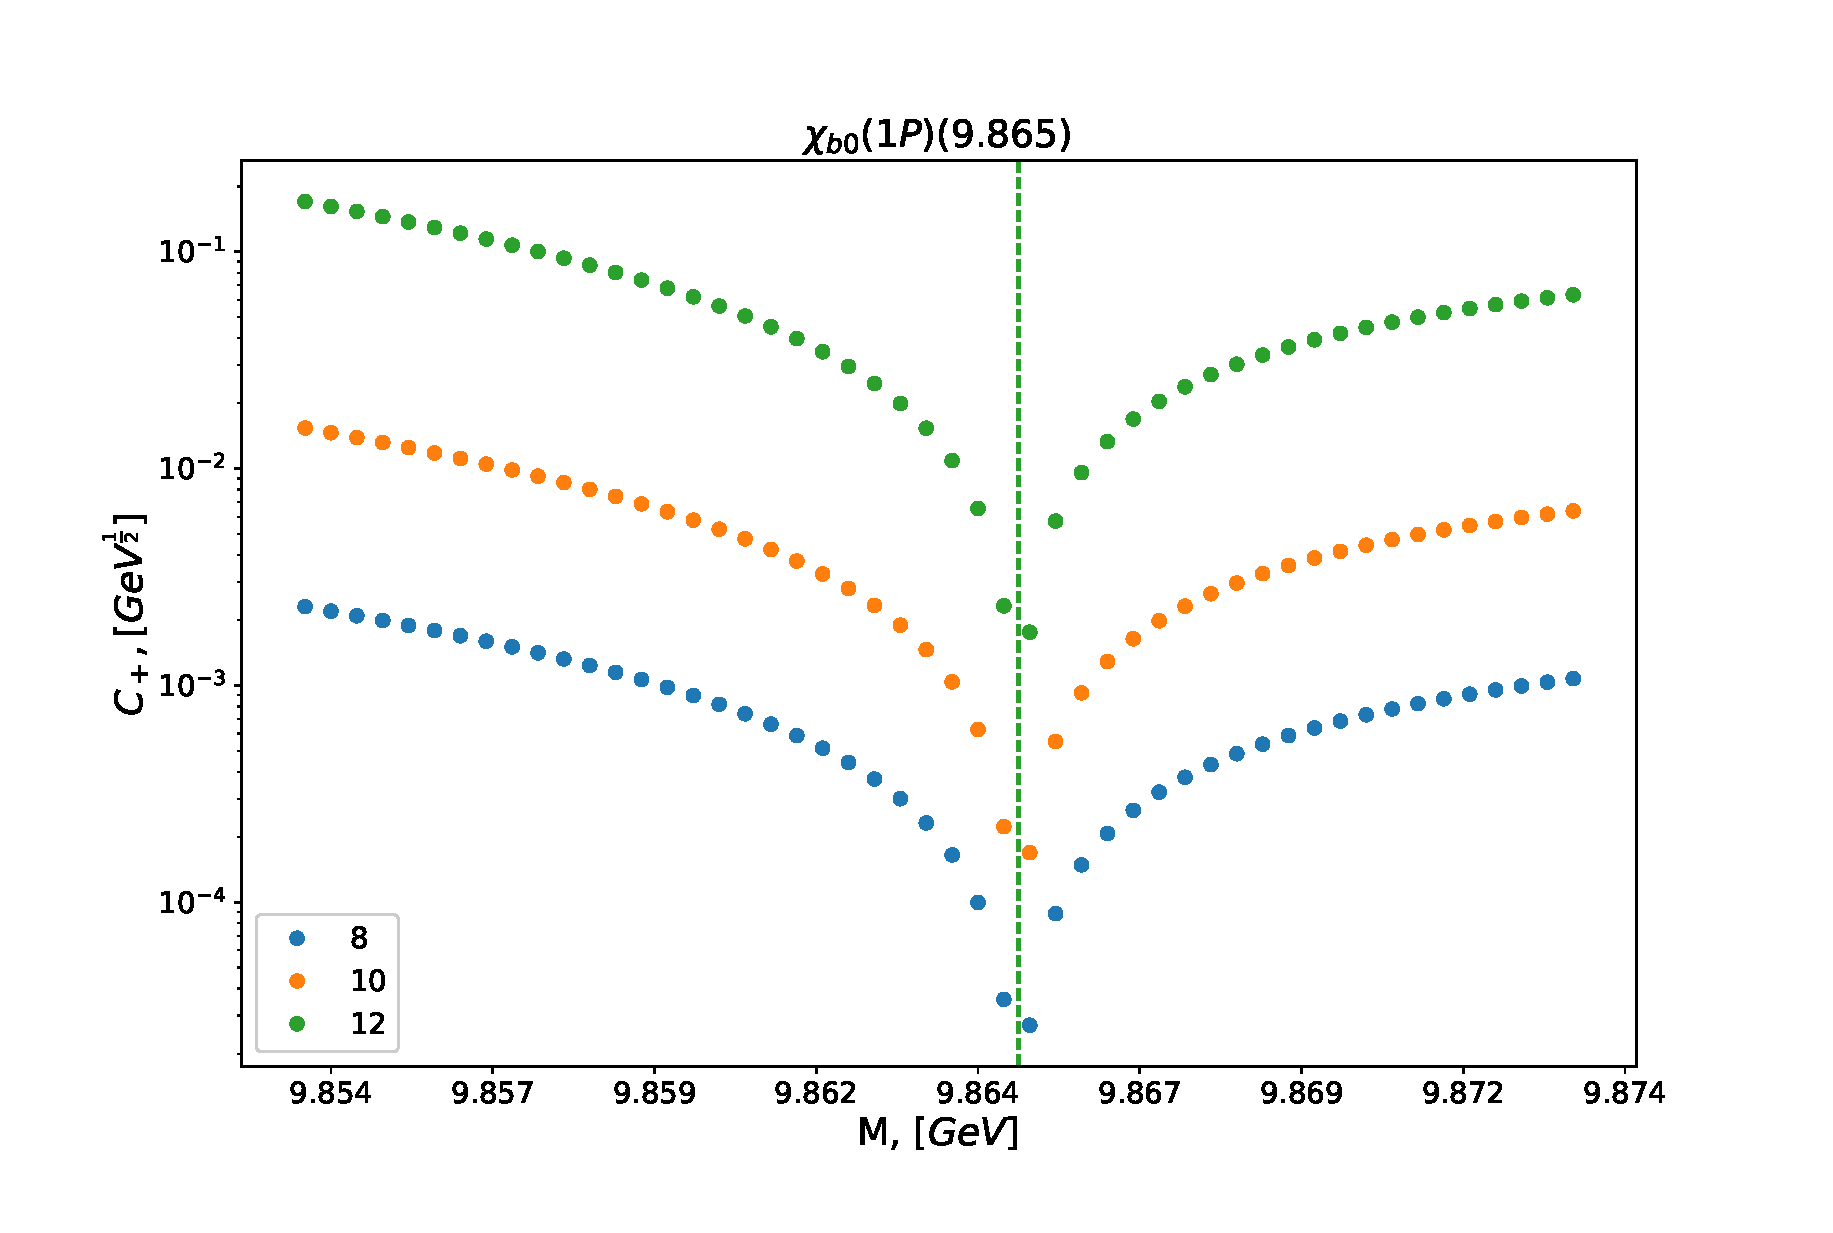
\includegraphics[width=15cm]{chi_b0_1P-dip.eps}
    \caption{Dependency of $C_+$ on mass in the screened potential for $\chi_{b0}(1P)$ (mass is directly related to the binding energy: $M = 2m_q + E_{binding}$). Damping used here is $10^{10}$} \label{fig:chib01P-dip}
\end{figure}

\begin{table}[H]
    \begin{tabular}{lr}
\toprule
{} &  Deviation from the highest cutoff [$GeV$] \\
Cutscale [$GeV^{-1}$] &                                            \\
\midrule
8                     &                               7.543720e-09 \\
10                    &                               1.863004e-11 \\
12                    &                               0.000000e+00 \\
\bottomrule
\end{tabular}

    \caption{Test of the accuracy ($\chi_{b0}(1P)$ with $10^{10}$ damping) in the screened potential} \label{tab:chib01P-dipcheck}
\end{table}

According to the method, value of $C_+$ should be evaluated at infinity. This is impossible in numerical calculations so cutoff has been introduced. To determine whether it is far enough we test how the eigenvalue depends on several of them. Different lines on~\cref{fig:chib01P-dip} are responsible for that. We also provide quantitative estimations for the same dip. As we assume, the highest cutoff provides the best result, we look at deviation from it. From the~\cref{tab:chic01P-dipcheck} it can be concluded, that accuracy is of order $\approx 10^{-10}~GeV = 0.1~eV$.

For comparison we provide the same plots for charmonium in screened and linear potential.

\begin{figure}[H]
    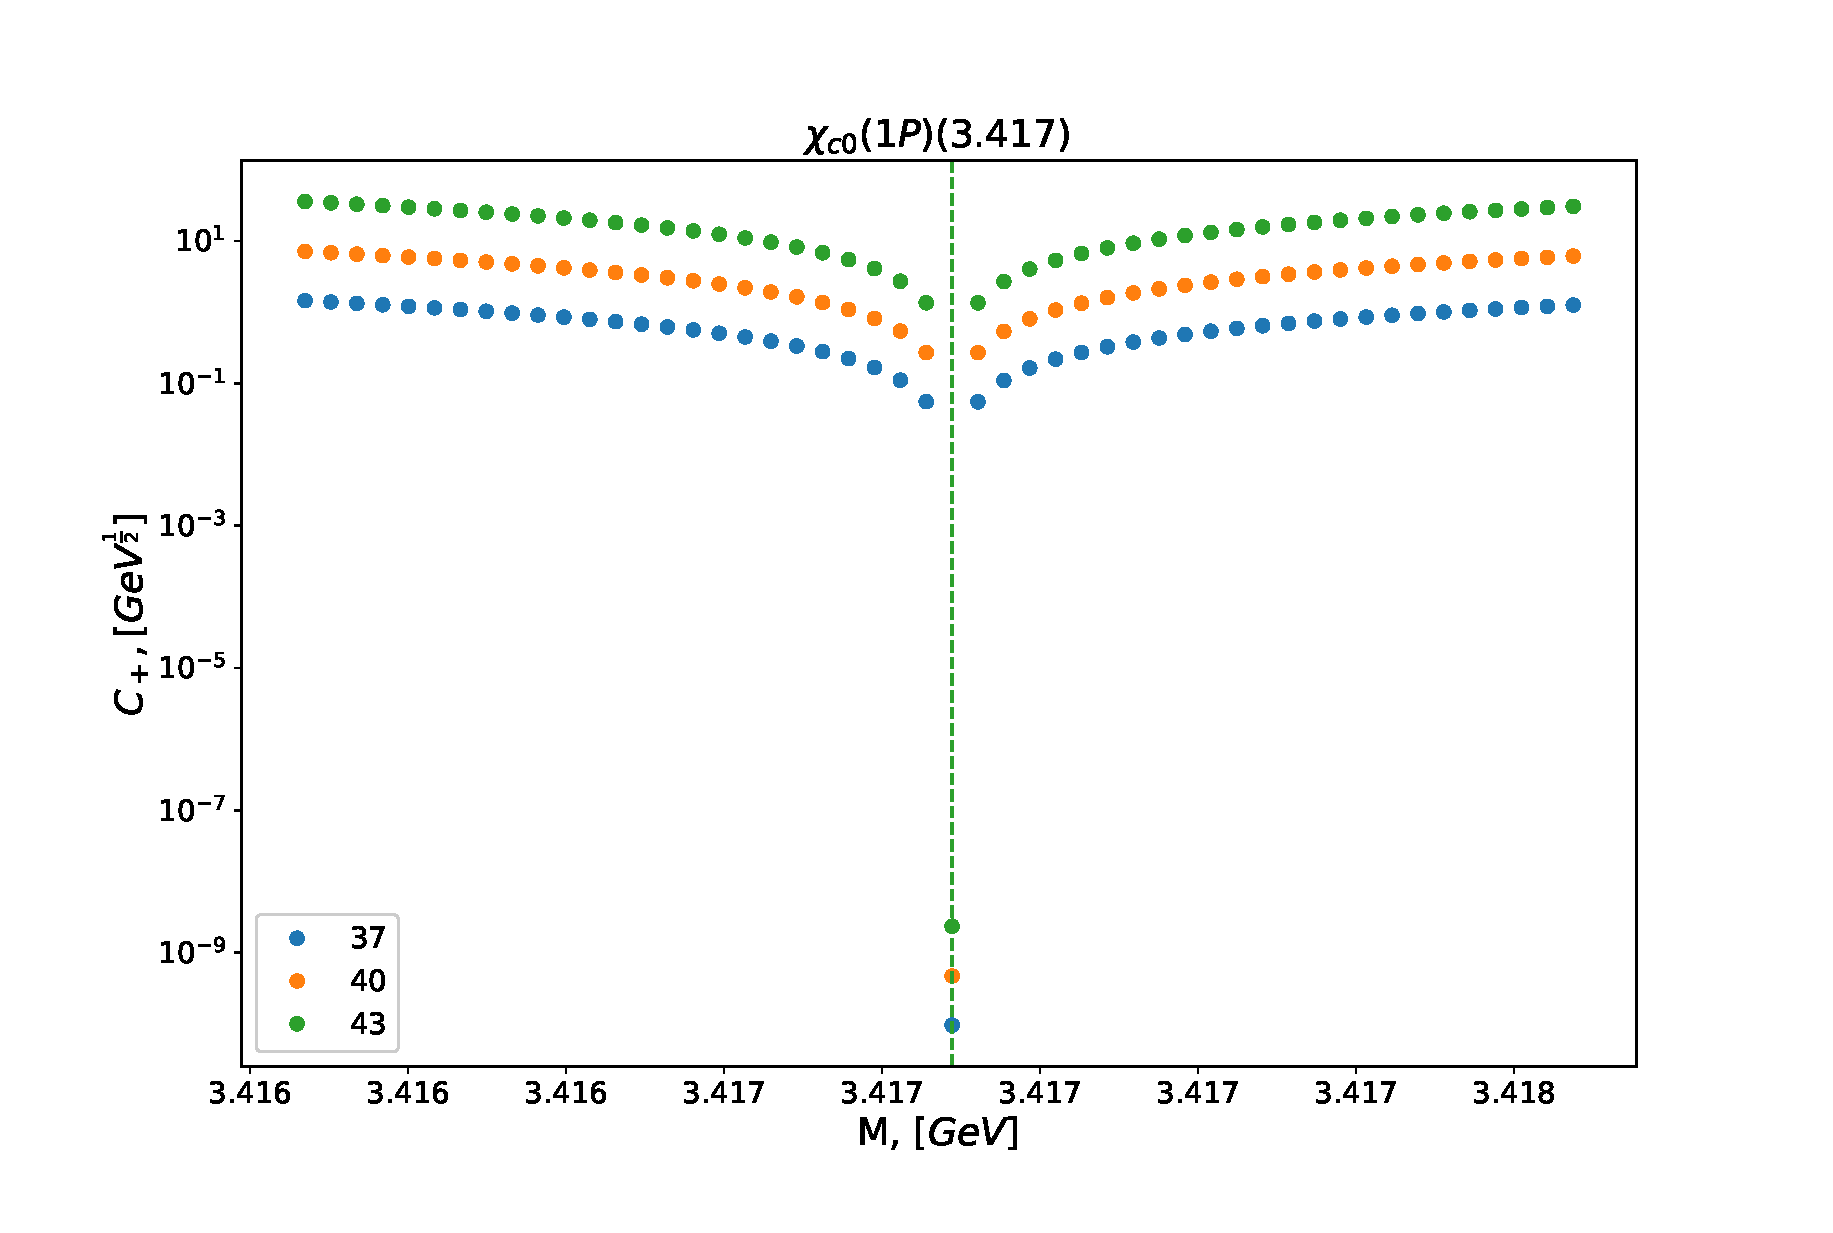
\includegraphics[width=15cm]{chi_c0_1P-dip.eps}
    \caption{Dependency of $C_+$ on mass in the screened potential for $\chi_{c0}(1P)$. Damping used here is $10^{10}$} \label{fig:chic01P-dip}
\end{figure}

\begin{table}[H]
    \begin{tabular}{lr}
\toprule
{} &  Deviation from the highest cutoff [$GeV$] \\
Cutscale [$GeV^{-1}$] &                                            \\
\midrule
    \begin{tabular}{l}
        37 \\ 40 \\ 43
    \end{tabular}       & eigenvalue doesn't change at least in 12th digit ($\approx 10^{-12}$) \\
\bottomrule
\end{tabular}

    \caption{Test of the accuracy ($\chi_{c0}(1P)$ with $10^{10}$ damping) in the screened potential} \label{tab:chic01P-dipcheck}
\end{table}

\begin{figure}[H]
    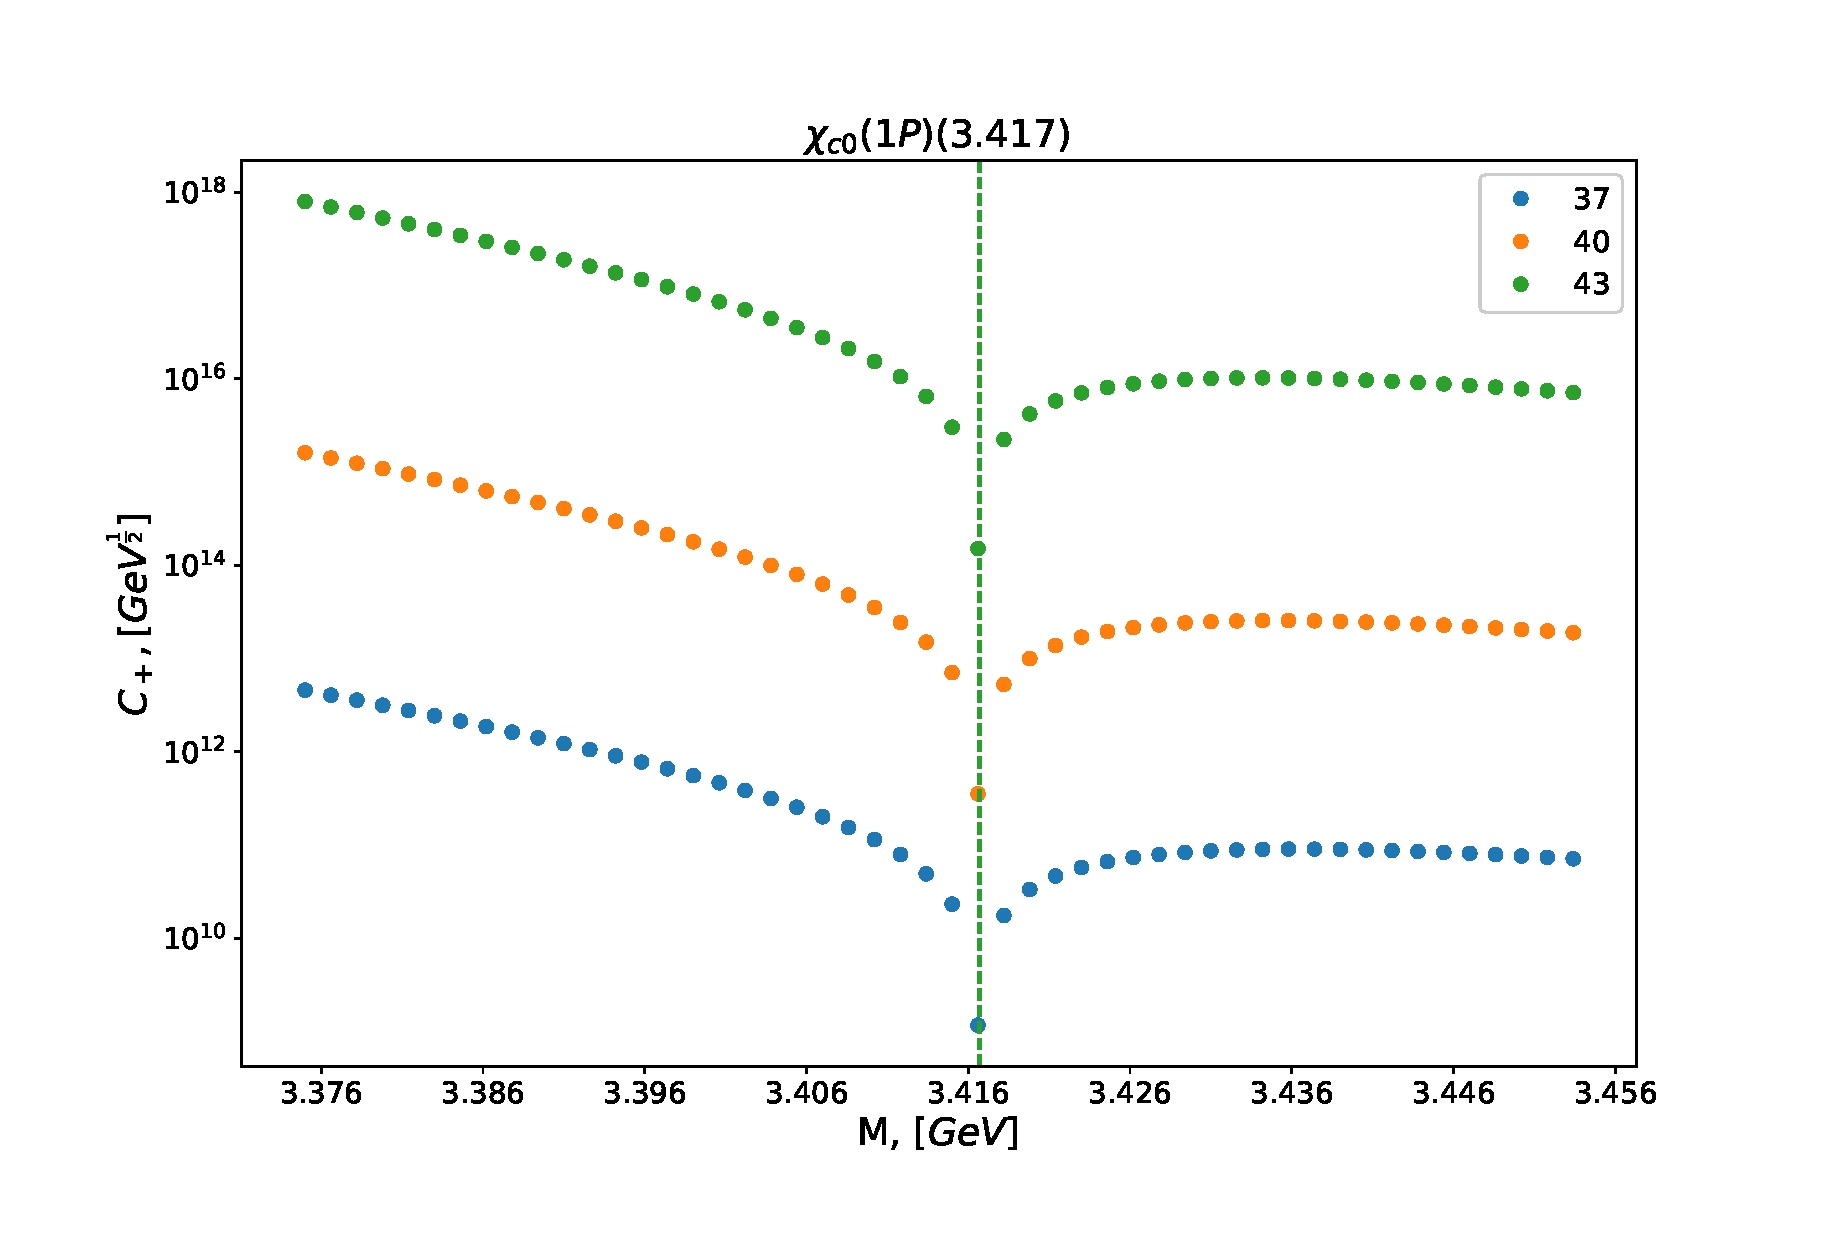
\includegraphics[width=15cm]{chi_c0_1P-lin-dip.eps}
    \caption{Dependency of $C_+$ on mass in the linear potential for $\chi_{c0}(1P)$. Damping used here is $10^{4}$} \label{fig:chic01P-lin-dip}
\end{figure}

\begin{table}[H]
    \begin{tabular}{lr}
\toprule
{} &  Deviation from the highest cutoff [$GeV$] \\
Cutscale [$GeV^{-1}$] &                                            \\
\midrule
37                    &                               1.736358e-06 \\
40                    &                              -1.840293e-08 \\
43                    &                               0.000000e+00 \\
\bottomrule
\end{tabular}

    \caption{Test of the accuracy ($\chi_{c0}(1P)$ with $10^{4}$ damping) in the linear potential} \label{tab:chic01P-lin-dipcheck}
\end{table}

What is significant for linear potential, in spite of comparable accuracy (to screening potential) magnitude far from origin differs by powers of ten. The same happens to the cutoff distance. One should go four times farther to gain comparable precision.

After the analysis of a particular state, we are ready to present big picture. We show Deng et al.~\cite{deng-charm,deng-bot} and our results show the same standard deviation compared to PDG~\cite{pdg}. There is nothing surprising here because we used parameters fitted by Deng.

\begin{table}[H]
    \caption{Bottomonium spectrum. Masses provided in $KeV$s. Standard deviation of Deng et al.~\cite{deng-bot} and our result from PDG~\cite{pdg} are comparable and $\approx 20KeV$. (Bottomonium provided as a test so states without experimental data were skipped. See entire table in appendix(\cref{sec:app:bot-spectrum}))}
    \begin{tabular}{lccc}
\toprule
{} &    PDG &   Deng &       Our \\
States             &        &        &           \\
\midrule
$\Upsilon(1S)$     &   9460 &   9460 &   9460.17 \\
$\eta_{b}(1S)$     &   9398 &   9390 &   9389.24 \\
$\Upsilon(2S)$     &  10023 &  10015 &  10015.45 \\
$\eta_{b}(2S)$     &   9999 &   9990 &   9989.87 \\
$\Upsilon(3S)$     &  10355 &  10343 &  10343.43 \\
%$\eta_{b}(3S)$     &      — &  10326 &  10326.08 \\
$\Upsilon(4S)$     &  10579 &  10597 &  10597.87 \\
%$\eta_{b}(4S)$     &      — &  10584 &  10584.28 \\
$\Upsilon(5S)$     &  10889 &  10811 &  10811.67 \\
%$\eta_{b}(5S)$     &      — &  10800 &  10800.36 \\
$\Upsilon(6S)$     &  10992 &  10997 &  10998.22 \\
%$\eta_{b}(6S)$     &      — &  10988 &  10988.49 \\
$\chi_{b2}(1P)$    &   9912 &   9921 &   9921.65 \\
$\chi_{b1}(1P)$    &   9893 &   9903 &   9903.28 \\
$\chi_{b0}(1P)$    &   9859 &   9864 &   9865.03 \\
$h_{b}(1P)$        &   9899 &   9909 &   9909.37 \\
$\chi_{b2}(2P)$    &  10269 &  10264 &  10264.22 \\
$\chi_{b1}(2P)$    &  10255 &  10249 &  10249.82 \\
$\chi_{b0}(2P)$    &  10233 &  10220 &  10220.83 \\
$h_{b}(2P)$        &  10260 &  10254 &  10254.13 \\
%$\chi_{b2}(3P)$    &      — &  10528 &  10528.24 \\
$\chi_{b1}(3P)$    &  10512 &  10515 &  10515.80 \\
%$\chi_{b0}(3P)$    &      — &  10490 &  10491.40 \\
%$h_{b}(3P)$        &      — &  10519 &  10519.29 \\
%$\Upsilon_{3}(1D)$ &      — &  10157 &  10157.60 \\
$\Upsilon_{2}(1D)$ &  10164 &  10153 &  10153.62 \\
%$\Upsilon_{1}(1D)$ &      — &  10146 &  10146.96 \\
%$\eta_{b2}(1D)$    &      — &  10153 &  10154.29 \\
%$\Upsilon_{3}(2D)$ &      — &  10436 &  10436.34 \\
%$\Upsilon_{2}(2D)$ &      — &  10432 &  10432.33 \\
%$\Upsilon_{1}(2D)$ &      — &  10425 &  10425.99 \\
%$\eta_{b2}(2D)$    &      — &  10432 &  10433.06 \\
%$h_{b3}(1F)$       &      — &  10339 &  10340.14 \\
%$\chi_{b4}(1F)$    &      — &  10340 &  10340.62 \\
%$\chi_{b3}(1F)$    &      — &  10340 &  10340.41 \\
%$\chi_{b2}(1F)$    &      — &  10338 &  10338.77 \\
\bottomrule
\end{tabular}

\end{table}

\begin{table} \begin{floatrow}
\floatbox[\capbot]{table}[\FBwidth]
    {\caption{Charmonium spectrum in screened potential. Masses provided in $KeV$s. Standard deviation of Deng et al.~\cite{deng-bot} and our result from PDG~\cite{pdg} are comparable and $\approx 43KeV$ }}
    {\begin{tabular}{lccc}
\toprule
{} &   PDG &  Deng &      Our \\
States          &       &       &          \\
\midrule
$\psi(1S)$      &  3097 &  3097 &  3096.86 \\
$\eta_{c}(1S)$  &  2984 &  2984 &  2983.99 \\
$\psi(2S)$      &  3686 &  3679 &  3678.97 \\
$\eta_{c}(2S)$  &  3639 &  3637 &  3637.32 \\
$\psi(3S)$      &  4040 &  4030 &  4029.68 \\
$\eta_{c}(3S)$  &     — &  4004 &  4004.23 \\
$\psi(4S)$      &  4415 &  4281 &  4281.27 \\
$\eta_{c}(4S)$  &     — &  4264 &  4263.62 \\
$\psi(5S)$      &     — &  4472 &  4471.42 \\
$\eta_{c}(5S)$  &     — &  4459 &  4458.53 \\
$\chi_{c2}(1P)$ &  3556 &  3553 &  3553.15 \\
$\chi_{c1}(1P)$ &  3511 &  3521 &  3521.44 \\
$\chi_{c0}(1P)$ &  3415 &  3415 &  3416.86 \\
$h_{c}(1P)$     &  3525 &  3526 &  3526.16 \\
$\chi_{c2}(2P)$ &  3927 &  3937 &  3937.36 \\
$\chi_{c1}(2P)$ &     — &  3914 &  3913.87 \\
$\chi_{c0}(2P)$ &  3918 &  3848 &  3849.64 \\
$h_{c}(2P)$     &     — &  3916 &  3915.94 \\
$\chi_{c2}(3P)$ &     — &  4211 &  4210.45 \\
$\chi_{c1}(3P)$ &     — &  4192 &  4192.05 \\
$\chi_{c0}(3P)$ &     — &  4146 &  4146.65 \\
$h_{c}(3P)$     &     — &  4193 &  4193.23 \\
$\psi_{3}(1D)$  &     — &  3808 &  3808.14 \\
$\psi_{2}(1D)$  &  3823 &  3807 &  3807.00 \\
$\psi_{1}(1D)$  &  3778 &  3792 &  3792.31 \\
$\eta_{c2}(1D)$ &     — &  3805 &  3805.11 \\
$\psi_{3}(2D)$  &     — &  4112 &  4112.38 \\
$\psi_{2}(2D)$  &     — &  4109 &  4109.20 \\
$\psi_{1}(2D)$  &  4191 &  4095 &  4095.19 \\
$\eta_{c2}(2D)$ &     — &  4108 &  4108.22 \\
$\psi_{3}(3D)$  &     — &  4340 &  4340.27 \\
$\psi_{2}(3D)$  &     — &  4340 &  4336.52 \\
$\psi_{1}(3D)$  &     — &  4324 &  4324.12 \\
$\eta_{c2}(3D)$ &     — &  4336 &  4335.98 \\
\bottomrule
\end{tabular}
}
\hspace{1cm}
\floatbox[\capbot]{table}[\FBwidth]
    {\caption{Charmonium spectrum in linear potential. Masses provided in $KeV$s. Standard deviation of Deng et al.~\cite{deng-bot} and our reslut from PDG~\cite{pdg} are comparable and $\approx 24KeV$ }}
    {\begin{tabular}{lccc}
\toprule
{} &   PDG &  Deng &      Our \\
States          &       &       &          \\
\midrule
$\psi(1S)$      &  3097 &  3097 &  3097.08 \\
$\eta_{c}(1S)$  &  2984 &  2983 &  2983.38 \\
$\psi(2S)$      &  3686 &  3679 &  3678.51 \\
$\eta_{c}(2S)$  &  3639 &  3635 &  3634.53 \\
$\psi(3S)$      &  4040 &  4078 &  4078.04 \\
$\eta_{c}(3S)$  &     — &  4048 &  4047.70 \\
$\psi(4S)$      &  4415 &  4412 &  4412.25 \\
$\eta_{c}(4S)$  &     — &  4388 &  4388.22 \\
$\psi(5S)$      &     — &  4711 &  4709.71 \\
$\eta_{c}(5S)$  &     — &  4690 &  4689.45 \\
$\chi_{c2}(1P)$ &  3556 &  3552 &  3551.80 \\
$\chi_{c1}(1P)$ &  3511 &  3516 &  3515.76 \\
$\chi_{c0}(1P)$ &  3415 &  3415 &  3416.69 \\
$h_{c}(1P)$     &  3525 &  3522 &  3522.10 \\
$\chi_{c2}(2P)$ &  3927 &  3967 &  3966.45 \\
$\chi_{c1}(2P)$ &     — &  3937 &  3937.28 \\
$\chi_{c0}(2P)$ &  3918 &  3869 &  3870.47 \\
$h_{c}(2P)$     &     — &  3940 &  3939.78 \\
$\chi_{c2}(3P)$ &     — &  4310 &  4309.96 \\
$\chi_{c1}(3P)$ &     — &  4284 &  4284.27 \\
$\chi_{c0}(3P)$ &     — &  4230 &  4231.02 \\
$h_{c}(3P)$     &     — &  4285 &  4285.23 \\
$\psi_{3}(1D)$  &     — &  3811 &  3811.44 \\
$\psi_{2}(1D)$  &  3823 &  3807 &  3806.55 \\
$\psi_{1}(1D)$  &  3778 &  3787 &  3787.06 \\
$\eta_{c2}(1D)$ &     — &  3806 &  3805.66 \\
$\psi_{3}(2D)$  &     — &  4172 &  4171.25 \\
$\psi_{2}(2D)$  &     — &  4165 &  4164.16 \\
$\psi_{1}(2D)$  &  4191 &  4144 &  4143.33 \\
$\eta_{c2}(2D)$ &     — &  4164 &  4163.71 \\
$\psi_{3}(3D)$  &     — &  4486 &  4486.38 \\
$\psi_{2}(3D)$  &     — &  4478 &  4477.97 \\
$\psi_{1}(3D)$  &     — &  4456 &  4456.67 \\
$\eta_{c2}(3D)$ &     — &  4478 &  4477.70 \\
\bottomrule
\end{tabular}
}
\end{floatrow} \end{table}

Having obtained mass spectrum of charmonium and bottomonium states it is interesting to compare wave functions. For qualitative presentation of the output we show our wave-functions overlayed onto plots presented by Deng et al.~\cite{deng-bot,deng-charm}:

\begin{figure}[H] \begin{floatrow}
    \ffigbox[\Xhsize]
        {\caption{Bottomonium S-states. (background from~\cite{deng-bot})}}
        {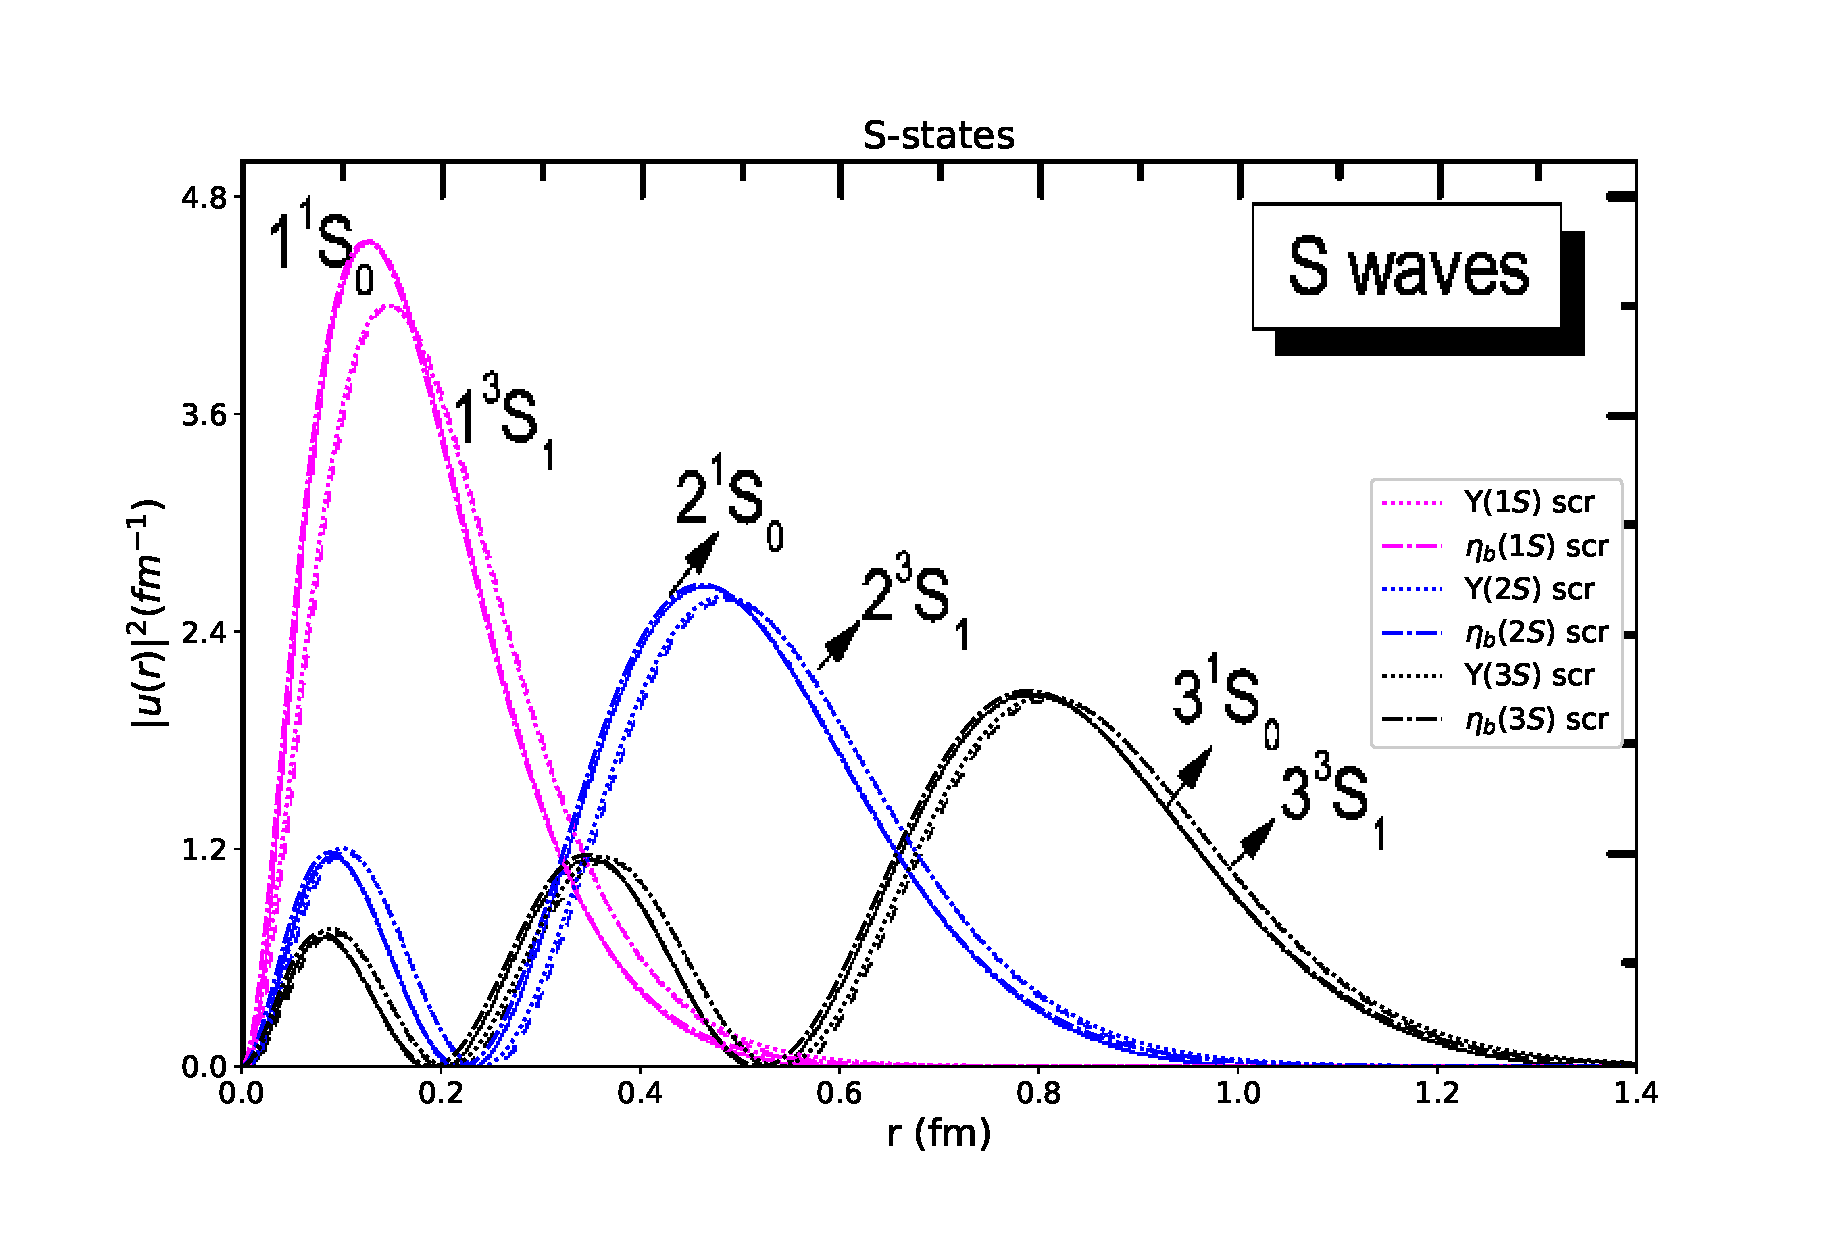
\includegraphics[width=10cm]{bot-s.eps}}
\end{floatrow} \end{figure}
 
For charmonium picture is the same:

\begin{figure}[H] \begin{floatrow}
    \ffigbox[\Xhsize]
        {\caption{Charmonium S-states. (background from~\cite{deng-charm})}}
        {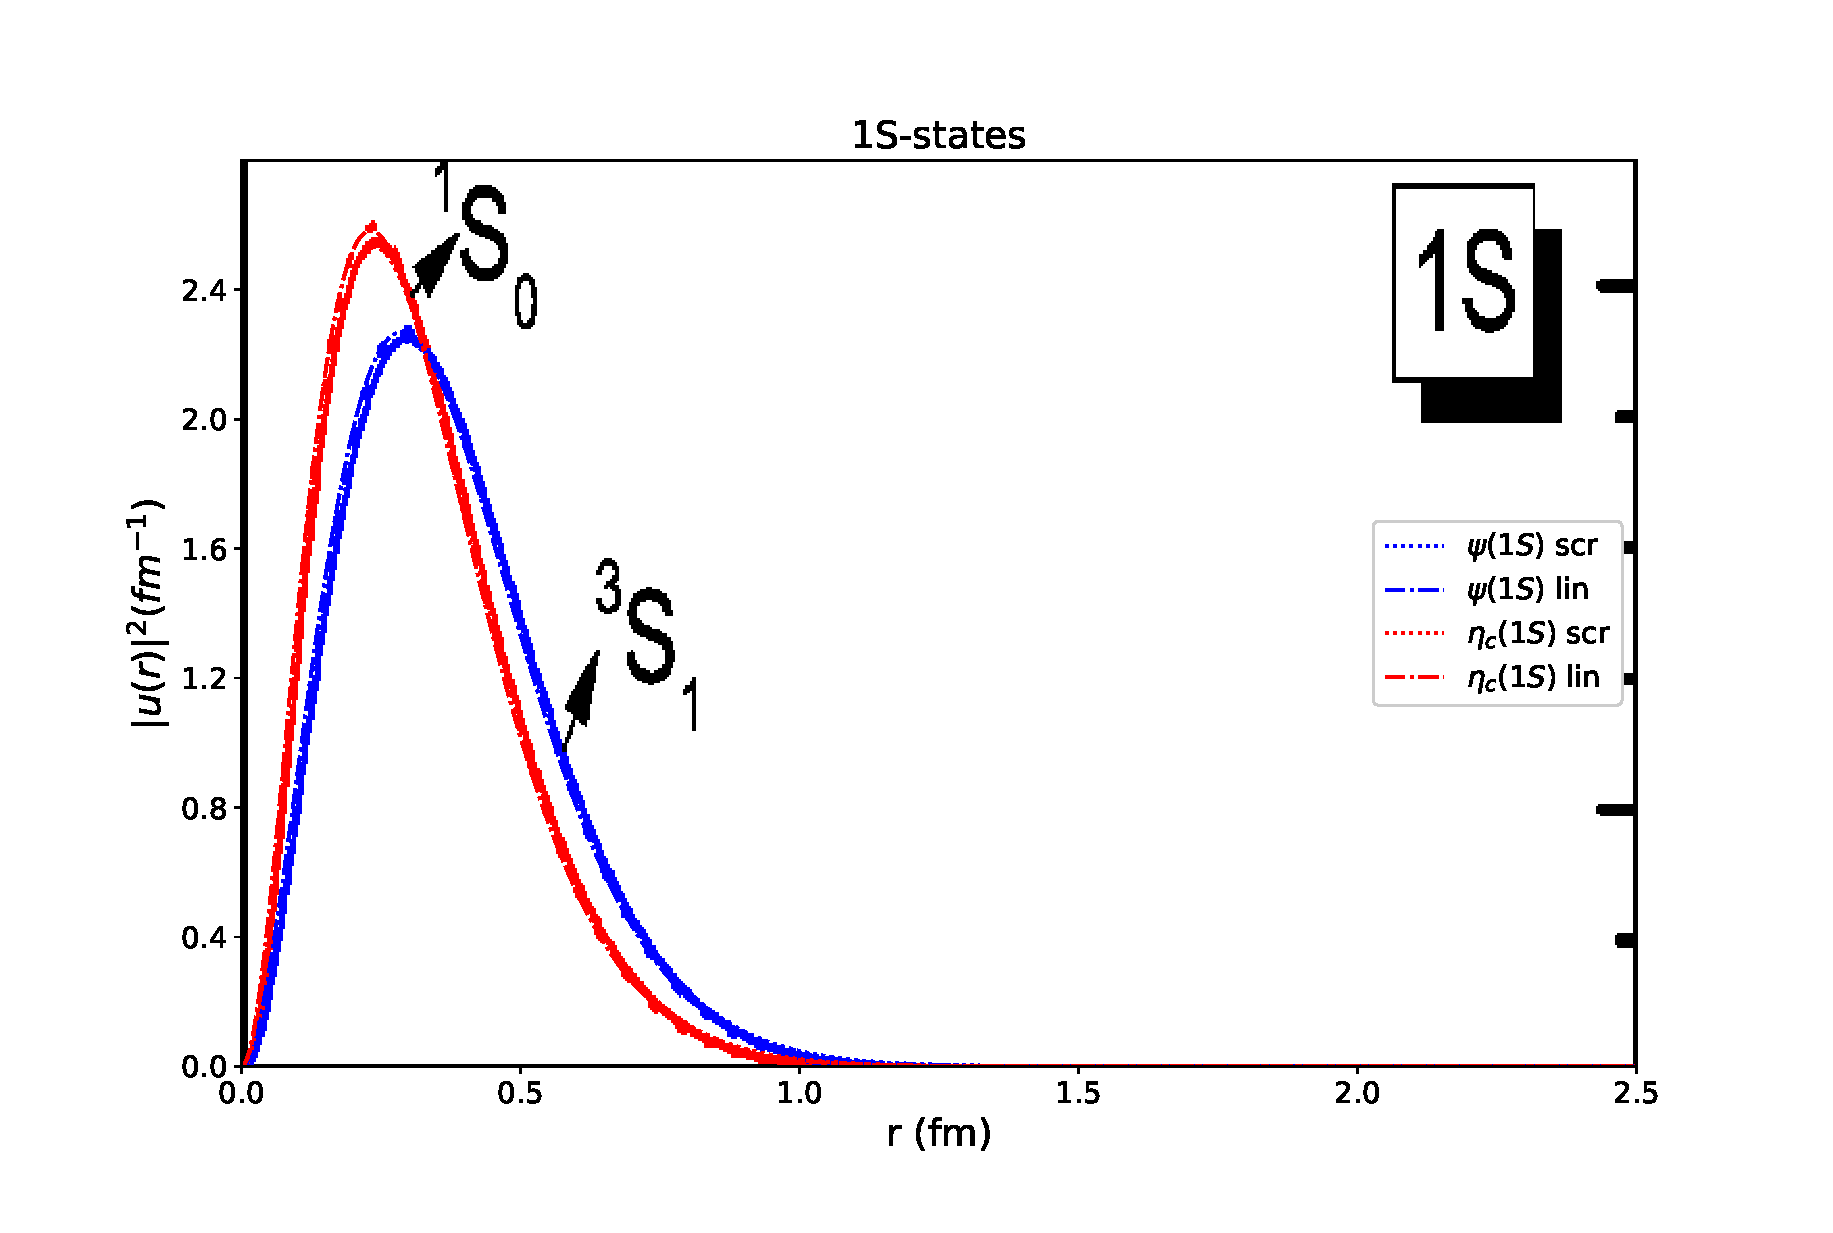
\includegraphics[width=10cm]{charm-1s.eps}}
\end{floatrow} \end{figure}

Such an analysis is a convenient way to make sure that wave functions don't gain enormous error at infinity where they should be damped. Moreover, the fact that linear potential grows unlimitedly can be traced for states with high orbital momenta. One can notice dashed lines representing linear case are shifted closer to the origin:

\begin{figure}[H] \begin{floatrow}
\ffigbox[\Xhsize]
    {\caption{Charmonium D-states. (background from~\cite{deng-charm})}}
    {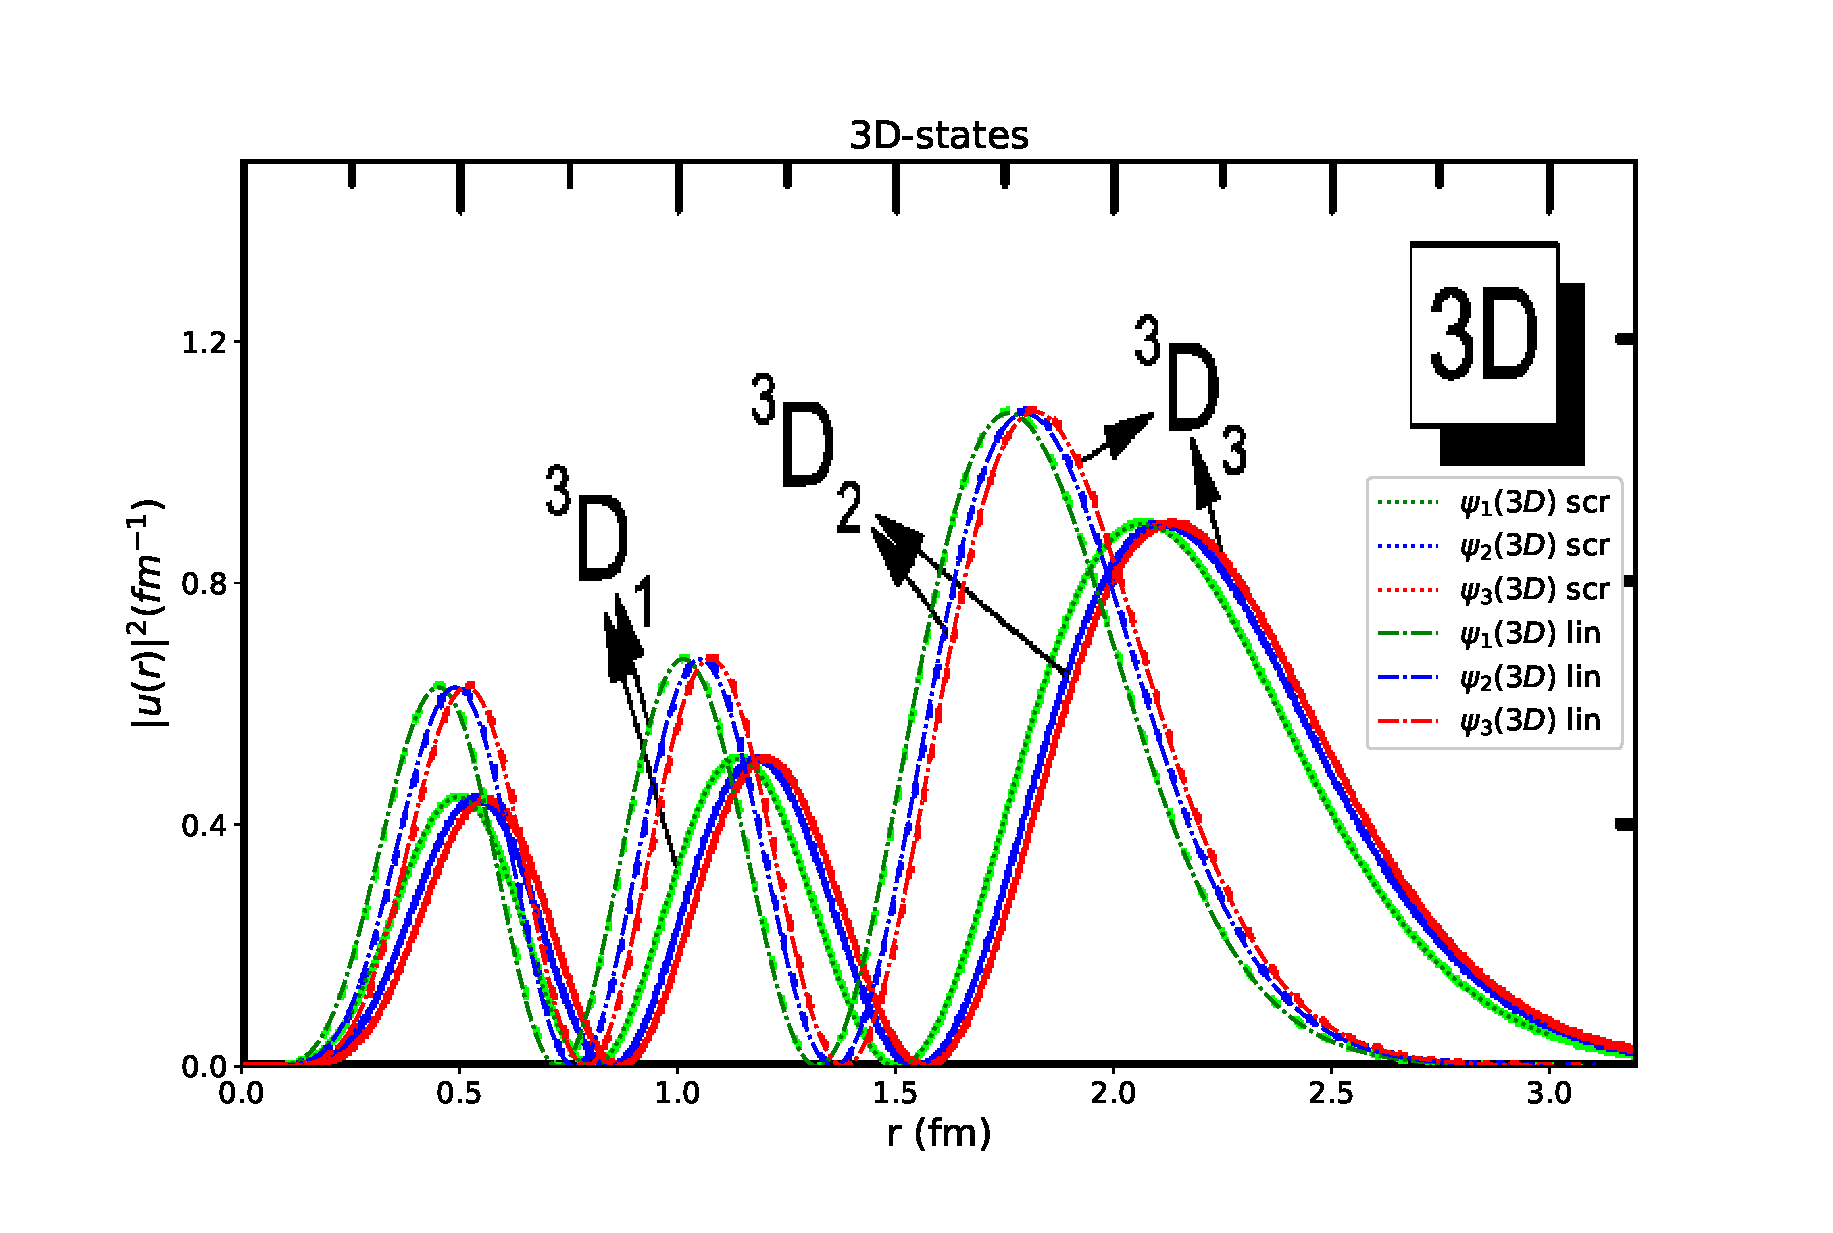
\includegraphics[width=10cm]{charm-3d.eps}}
\end{floatrow} \end{figure}
